\documentclass[crop,tikz]{standalone}                 
\usepackage{physics}

\makeatletter                                                                                        

\newcommand{\sq}[1]{\frac{1}{\sqrt{#1}}}

\begin{document}

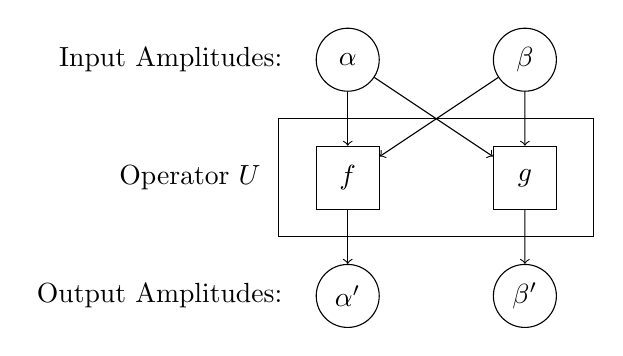
\begin{tikzpicture}[scale=1.5]                                                                          
\usetikzlibrary{positioning}
% tikz code here
%\draw [dashed] (0,0) grid (2,2);

% Input amplitudes
\node (a0) [draw, circle, minimum size=0.80cm] at ( 0.00, 2.00) {$\alpha$};
\node (b0) [draw, circle, minimum size=0.80cm] at ( 1.50, 2.00) {$\beta$};
\node (in) [left = 0.30cm of a0] {Input Amplitudes:};

% Functions
\node (f)  [draw, rectangle, minimum size=0.80cm] at ( 0.00, 1.00) {$f$};
\node (g)  [draw, rectangle, minimum size=0.80cm] at ( 1.50, 1.00) {$g$};

% Operator U
\node (u) [draw, rectangle, minimum width=4.00cm, minimum height=1.50cm] at ( 0.750, 1.00) {$$};
\node (ul) [left = 0.10cm of u] {Operator $U$};

% Output amplitudes
\node (a1) [draw, circle, minimum size=0.80cm] at ( 0.00, 0.00) {$\alpha'$};
\node (b1) [draw, circle, minimum size=0.80cm] at ( 1.50, 0.00) {$\beta'$};
\node (ot) [left = 0.30cm of a1] {Output Amplitudes:};

% Connections
\draw [->] (a0) -- (f);
\draw [->] (a0) -- (g);
\draw [->] (b0) -- (f);
\draw [->] (b0) -- (g);
\draw [->] (f) -- (a1);
\draw [->] (g) -- (b1);

\end{tikzpicture}                                                                                    

\end{document}
